\documentclass[letterpaper,twocolumn,openany,nodeprecatedcode]{dndbook}

% Use babel or polyglossia to automatically redefine macros for terms
% Armor Class, Level, etc...
% Default output is in English; captions are located in lib/dndstring-captions.sty.
% If no captions exist for a language, English will be used.
%1. To load a language with babel:
%	\usepackage[<lang>]{babel}
%2. To load a language with polyglossia:
%	\usepackage{polyglossia}
%	\setdefaultlanguage{<lang>}
\usepackage[italian]{babel}
%\usepackage[italian]{babel}
% For further options (multilanguage documents, hypenations, language environments...)
% please refer to babel/polyglossia's documentation.
\usepackage[utf8]{inputenc}
\usepackage[singlelinecheck=false]{caption}
\usepackage{lipsum}
\usepackage{listings}
\usepackage{shortvrb}
\usepackage{stfloats}
\usepackage{graphicx}% http://ctan.org/pkg/graphicx


\captionsetup[table]{labelformat=empty,font={sf,sc,bf,},skip=0pt}

\MakeShortVerb{|}

\lstset{%
  basicstyle=\ttfamily,
  language=[LaTeX]{TeX},
  breaklines=true,
}

\title{I corrieri della Grancontessa \\
\large OneShot di D\&D 5e per 4 o 6 giocatori di 4$^\circ$ livello}
\author{}
\date{2024/06/01}

\begin{document}

\frontmatter

\maketitle

\tableofcontents


\mainmatter%




%%%%%%%%%%%%%%% TEMPLATE %%%%%%%%%%%%%%%%%%%%%%%%

\chapter{Introduzione}

\section{Chi siamo}
\DndDropCapLine{C}{aro Dungeon Master}, siamo un gruppo di appassionati di Dungeons \& Dragons che ha preparato questa avventura per te. Vorremmo condividere con te il nostro approccio al gioco di D\&D per darti alcuni suggerimenti su come condurre al meglio questa avventura.

Quando creiamo i nostri personaggi giocanti (PG), ci concentriamo sulla costruzione di personaggi complessi. Introduciamo difetti che possono aggiungere elementi divertenti al gioco, sviluppiamo background coerenti e integrati nell'ambientazione. Dedichiamo tempo a riflettere sui pensieri e le motivazioni dei PG, esplorando come reagirebbero a diverse situazioni. Ad esempio, durante la nostra ultima avventura, lo stregone Virgilio Monforte aveva problemi di memoria, mentre Clara Spina, la chierica, citava spesso proverbi senza senso. Prestiamo maggiore attenzione a questi aspetti rispetto alle regole specifiche di D\&D, che comunque consideriamo come punto di riferimento.

Quando un personaggio compie azioni che devono rimanere segrete dagli altri giocatori, utilizziamo Telegram per comunicare in modo riservato con il DM. Questa tecnica ha contribuito significativamente al divertimento di tutti in numerose occasioni. Nella OneShot descritta in questo testo, la comunicazione segreta con il DM è fondamentale per il successo dell'avventura.

Riteniamo che il DM debba avere una trama di base da seguire, ma sia importante saper improvvisare e adattarsi alle situazioni emergenti durante il gioco. Alla fine di questo testo, condivideremo un breve resoconto delle avventure vissute durante la nostra campagna.


\section{La oneshot}
Questa avventura è una OneShot basata sul gioco di ruolo Dungeons \& Dragons 5° edizione\cite{dnd:giocatore}, progettata per un gruppo di 4-6 giocatori di 4$^\circ$ livello. L'ambientazione si colloca nel Medioevo Italiano, nei pressi del Castello di Canossa, i cui resti si trovano nel basso Appennino Reggiano, in Italia. Elementi magici, razze, classi e altri aspetti fantasy tipici di D\&D vengono integrati nell'ambientazione storica, ad eccezione delle seguenti razze non presenti: dragonidi, tiefling e mezz'orchi.

I personaggi giocanti (PG) sono creati dal Dungeon Master (DM). Nel paragrafo relativo al background dei PG (§\ref{PG}) sono fornite linee guida per la creazione dei personaggi. Alcuni di questi elementi sono considerati cruciali per mantenere coerenza con la trama.

La missione, inizialmente semplice e lineare, dovrebbe evolversi in un momento di conflitto interno al gruppo poiché, come vedrai in seguito, uno dei PG avrà una missione segreta opposta al resto del gruppo.

Le creature incontrate durante questa OneShot sono evidenziate in \textbf{grassetto} e fanno riferimento al Manuale dei Mostri di D\&D 5e\cite{dnd:mostri}.



\section{Contesto storico}

Matilde di Canossa\footnote{Questo paragrafo è stato dedotto e sintetizzato dalla voce enciclopedica di Wikipedia "Matilde di Canossa"} (Fig. \ref{fig:matilde})\cite{wiki:matilde}, o più correttamente Matilde di Toscana, nota anche con lo pseudonimo di \textit{Magna Comitissa} in italiano Gran Contessa, nacque nel 1046, terzogenita della potentissima famiglia feudale italiana dei Canossa considerata all'epoca la più potente famiglia d'Europa. Trascorse i primi anni della sua esistenza nell'agiatezza e serenità del castello di Canossa, teatro dei grandi banchetti e delle sontuose feste organizzate dal padre. Tuttavia a soli sei anni Matilde assistette a un evento che avrebbe cambiato radicalmente il corso della sua vita: il 6 maggio 1052 il padre Bonifacio fu ucciso a tradimento durante una battuta di caccia da uno dei suoi vassalli, che lo trapassò alla gola con una freccia avvelenata. L'agonia del duca durò alcune ore; nella tarda serata dello stesso giorno egli spirò.

\begin{figure}
\centering
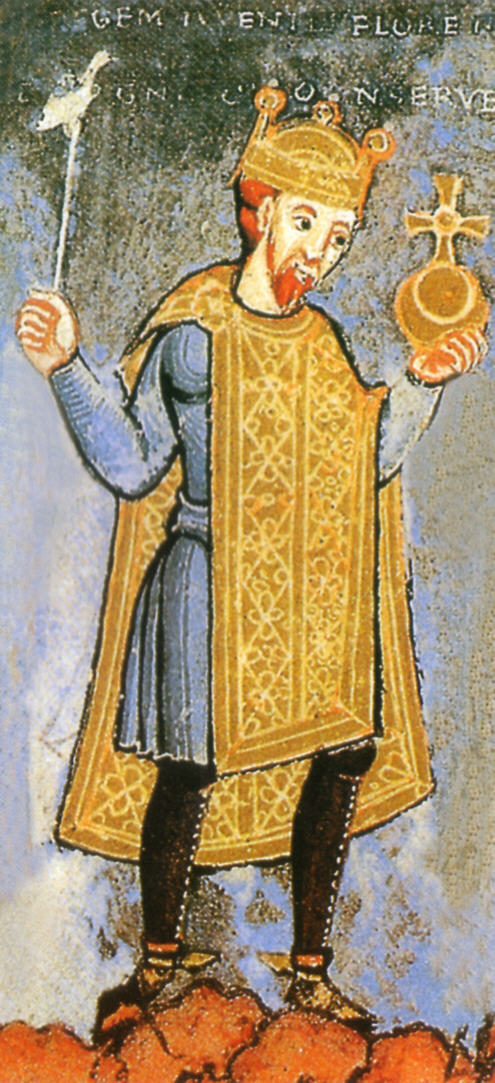
\includegraphics[width=9cm]{./img/enrico3.png}
\caption{Riproduzione di Enrico III. Immagine di Pubblico Dominio da Wikimedia Commons.}
\label{enrico3}
\end{figure}


Beatrice, la madre di Matilde, rimasta vedova con 3 figli piccoli in difficoltà nel reggere il ruolo del marito Bonifacio, capo di una casata così potente, cercò la protezione dell'imperatore Enrico III (Fig. \ref{enrico3}) il quale garantì questo privilegio per Matilde e i suoi fratelli.

Purtroppo i fratelli di Matilde perirono per un maleficio: avvelenamento.

La madre di Matilde era imparentata con il papa Leone IX che garantiva anch'egli una protezione alla casata dei Canossa. Gli equilibri fra potere temporale e potere spirituale permisero alla giovane Matilde e alla sua casata di trascorrere alcuni anni in relativa serenità.

Alla morte del papa Leone IX cambiarono gli equilibri e l'imperatore Enrico III prese in ostaggio Matilde e sua madre e le portò in Germania; ma dopo un anno anche Enrico III morì e così Matilde ritornò in Italia. La madre Beatrice cercò una nuova protezione risposandosi con Goffredo il Barbuto.

Goffredo il Barbuto, sposando Beatrice, era diventato signore della Tuscia. Una clausola del contratto di matrimonio stabilì che il figlio di Goffredo, detto Goffredo il Gobbo (Fig. \ref{fig:goffredo}), avrebbe sposato la figlia di Beatrice, Matilde, per consolidare il suo potere e quello dei Canossa.

Matilde e Goffredo il Gobbo si unirono in matrimonio nella Lorena Francese. Il marito era un giovane onesto e coraggioso, ma afflitto da alcuni difetti fisici (tra gli altri gozzo e gobba), comunque Matilde, conscia dei doveri nobiliari per i quali era stata educata e con la persuasione della madre, seppur riluttante restò in Francia coabitando con il marito e ne rimase incinta.

All'inizio del 1071 Matilde partorì una bambina che chiamò Beatrice, per poter rinnovare il nome della madre. Il parto però non fu facile e dopo pochi giorni la piccola Beatrice morì. La mamma di Matilde eresse il monastero di Frassinoro, nell'Appennino Modenese, per <<la grazia dell'anima della defunta Beatrice mia nipote>>.

Nei mesi successivi Matilde rischiò la vita, non solo per i postumi del parto difficile, ma anche per l'ira del casato di Lorena che accusò la Gran Contessa di portare il malocchio. Nel gennaio del 1072 Matilde fuggi dalla Lorena Francese per tornare nel Castello di Canossa con la madre.

Il 26 dicembre del 1073 i PG sono stati incaricati da Tobaldo Malatesta\footnote{Questo NPC non è realmente esistito}, fedele servitore di Matilde, di condurre un carro di provviste (salumi, formaggi, grano e vino) da Parma al Castello di Canossa entro il 28 dicembre. Inoltre è stata consegnata al paladino del gruppo  una pergamena, una cosiddetta \textit{rotula}, che dovrà consegnare personalmente a Matilde, proteggendo la segretezza della missiva a costo della vita. La rotula di pergamena è avvolta in una pezzo di pelle e sigillata con il simbolo di cera lacca della casata dei Canossa. 

\begin{figure}
\centering
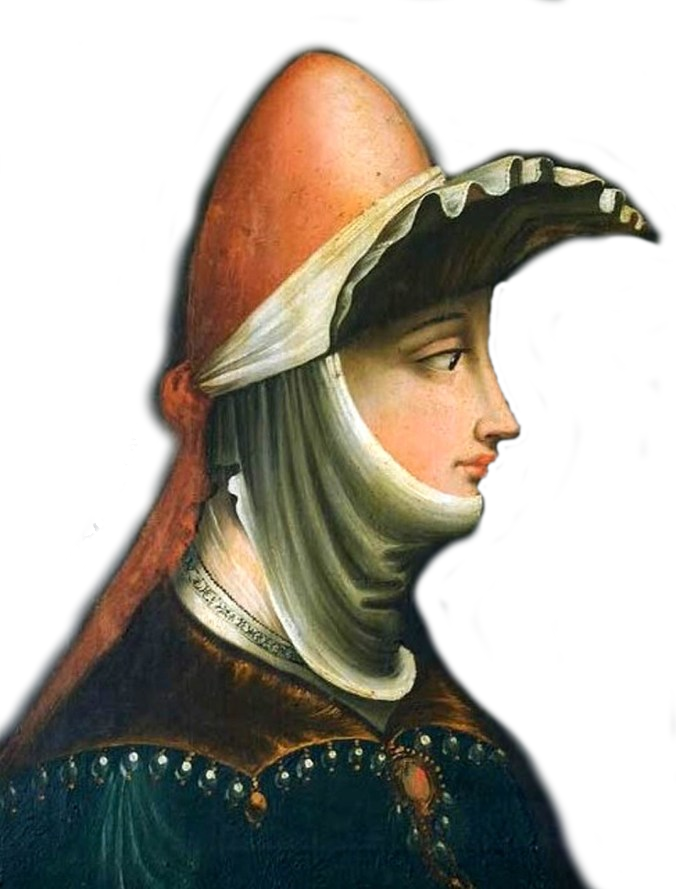
\includegraphics[width=7.5cm]{img/matilde.png}
    \caption{\textsf{Parmigianino, Ritratto di Matilde di Canossa, XVI secolo, Museo Diocesano, Mantova. Immagine di Pubblico Dominio da Wikimedia Commons.}}
    \label{fig:matilde}
\end{figure}

\begin{DndSidebar}{Quando fornire queste informazioni?}Il contesto storico descritto in questo paragrafo può essere presentato ai giocatori dal Dungeon Master nel momento ritenuto più opportuno. Durante la nostra partita a questa avventura, il DM ha utilizzato un avventore della locanda per trasmettere queste informazioni ai PG.
\end{DndSidebar}

\subsection{Eventi successivi}
A parte la missione dei PG e il personaggio di Tobaldo Malatesta, gli eventi storici menzionati sopra sono realmente accaduti. Di seguito viene descritto ciò che accadde a Matilde dopo il suo ritorno al Castello di Canossa. Questi avvenimenti non fanno parte dell'avventura stessa, ma possono essere utili al DM che desidera preparare questa OneShot, al fine di comprendere meglio l'idea alla base della storia.

Tra il 1073 e il 1074, il marito di Matilde, Goffredo il Gobbo, scese in Italia per riconquistarla offrendole terre e armate, ma la Grancontessa rifiutò con fermezza e determinazione. Il suo atteggiamento contribuì a creare il mito di una donna priva di debolezze.

Nel 1076, Goffredo il Gobbo cadde vittima di un'imboscata nelle sue terre vicino ad Anversa. Durante la notte, mentre si recava al gabinetto, un sicario in agguato gli conficcò una spada tra le natiche, lasciando l'arma conficcata nella ferita. Inizialmente sembrava che potesse sopravvivere, ma una settimana dopo, il 27 febbraio 1076, morì, lasciando Matilde vedova. Molti commentatori dell'epoca la accusarono di essere stata personalmente coinvolta nel crimine; tuttavia, il colpevole più probabile fu indicato come il conte fiammingo Roberto I delle Fiandre. In ogni caso, Matilde non offrì alcun sostegno finanziario alla Chiesa per l'anima del marito ucciso, né fece celebrare una messa o dedicò un convento in suo onore, come era consuetudine tra i nobili.

\begin{figure}
\centering
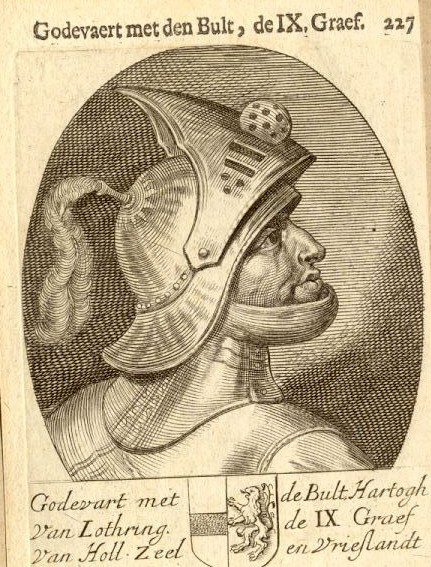
\includegraphics[width=7.5cm]{img/goffredo-il-gobbo.png}
    \caption{\textsf{Goffredo IV di Lorena detto ''il Gobbo''. Immagine di Pubblico Dominio da Wikimedia Commons.}}
    \label{fig:goffredo}
\end{figure}

\section{La missione}
È il 26 dicembre del 1073, i PG si trovano nella città di Parma dove sono stati incaricati da Tobaldo Malatesta, servitore di alto rango della casata dei Canossa, di scortare un carro di provviste destinate al Castello di Canossa. Il carro contiene prosciutti, salami, culatelli e forme di formaggio stagionato, che gli abati Benedettini di Parma hanno iniziato a produrre da alcuni mesi\footnote{L'origine del Parmigiano reggiano, secondo la voce enciclopedica di Wikipedia, avrebbe origine nel XII secolo nelle abbazie benedettine e cistercensi situate fra Reggio Emilia e Parma. Ci sembrava carino aggiungere a questa storia le origini del formaggio più famoso del mondo anche se in realtà nacque un po' dopo.}, destinati alla festa di fine anno che si svolgerà al castello. Oltre ai viveri, Tobaldo consegna una pergamena sigillata al paladino del gruppo, Dante Passafiume, che dovrà portare personalmente a Matilde e dovrà "proteggerne la segretezza anche a costo della propria vita".

Herbert Mann, il cui vero nome è Olin, avrà una missione segreta diversa dal resto del gruppo. Questo PG è un sicario incaricato da Roberto I delle Fiandre il quale lo ha pagato in anticipo 200 monete d'oro per uccidere Goffredo il Gobbo, \textbf{nobile} con 32 PF (Manuale dei Mostri p.349 \cite{dnd:mostri}) che, gli è stato detto, alloggia al Castello di Canossa. Il sicario è riuscito ad infiltrarsi nel gruppo di corrieri per il trasporto di viveri al Castello, tuttavia la sua missione è una missione omicida.

I PG partiranno da Parma per Canossa durante una tormenta di neve e saranno costretti a passare la notte a Plebs de Caviliano, oggi nota come San Polo d'Enza. Il giorno successivo durante il viaggio avranno alcuni attacchi e tentativi di furto.

Giunti al castello, consegneranno le provviste e la lettera a Matilde. Si renderanno conto solo in questo momento della vera missione di questa OneShot. La missiva informerà Matilde che qualcuno sta cercando di uccidere Goffredo. Matilde quindi incaricherà il gruppo di proteggere il Duca.

A questo punto i PG avranno l'incarico di protezione del nobile, ad esclusione del PG infiltrato che dovrà ucciderlo.


\section{PG in breve}\label{PG}

\paragraph{Isabella Grattaciotoli} Ha 28 anni, è una \textit{halfling ladra}. Non particolarmente forte ma molto abile a nascondersi e particolarmente agile. Orfana di entrambi i genitori ha accettato di partecipare a questa missione perché la ricompensa le permetterà di provvedere al sostegno dei suoi fratelli per tutto l'inverno. Difetti: quando vede dei dolci perde letteralmente la testa.

\paragraph{Dante Passafiume} (PG indispensabile) È un \textit{paladino umano} di 50 anni, un veterano che fa parte della rete di messaggeri. Una persona coraggiosa e dall'alta integrità morale. Dante, se prende un impegno, lo porta a termine. Difetti: si irrita quando viene contraddetto.

\paragraph{Caterina Portinari} Caterina ha 25 anni ed è la più giovane del gruppo. Viene da una famiglia benestante. I genitori avrebbero voluto educarla per diventare una signora, una damigella, ma lei è una donna di azione. Fuggita dalla famiglia, ha studiato per un paio d'anni armi e tattiche di combattimento e ora è un'abile \textit{guerriera umana}. Difetti: quando si tratta di finire un nemico esita.

\paragraph{Virgilio Monforte} È uno \textit{stregone mezz'elfo} anziano di 132 anni. Ha sempre messo i suoi innati poteri al servizio dei nobili del territorio. Difetti: a volte perde la testa e usa incantesimi totalmente inutili e ha problemi di perdita di memoria.

\paragraph{Clara Spina} Clara ha 35 anni, è una umana chierica, appartiene al dominio della vita, la sua missione è aiutare gli altri. Difetti: è una irrefrenabile pettegola.

\paragraph{Olin (nome di copertura Herbert Mann)} (PG indispensabile) È un \textit{umano ladro} di 43 anni ma ufficialmente bardo con uno strumento rotto. È un sicario infiltrato nel gruppo per uccidere Goffredo il Gobbo. Difetti: è irritato dai nobili altezzosi, anche se riesce a trattenersi, a volte la sua irritazione traspare.




\subsection{NPC in breve}

\paragraph{Tobaldo Malatesta} Servitore di alto rango di Matilde. Gentile, una persona abituata a comandare, conosce Dante Passafiume e ne riconosce il valore.

\paragraph{Filippo Pocaterra} Oste della Locanda del Cane Zoppo di San Polo d'Enza. Gentile ma non è la persona più pulita del regno. L'igiene non è la sua specialità (Fig.\ref{fig:oste}).

\paragraph{Matilde di Canossa} La Grancontessa ha 25 anni, ha la fama di essere una donna dura tutta di un pezzo, ma probabilmente è più debole di quello che sembra.

\paragraph{Goffredo il Gobbo} Ha una vistosa gobba ma di fatto è una persona massiccia che sa difendersi. Non è la persona più simpatica del mondo. È venuto in Italia per riconquistare Matilde promettendole terre. Quest'ultima lo ha rifiutato. Considera Matilde una lurida sgualdrina.


\chapter{L'arrivo al villaggio}
\DndDropCapLine{I}{ PG stanno trasportando} un carico di viveri e una pergamena con un messaggio segreto da consegnare di persona a Matilde. La missiva è in custodia al paladino che deve difenderla a costo della vita. Il DM potrebbe decidere di non rivelare subito la missione, ma farla scoprire più lentamente con un flashback e leggere il testo seguente.

\begin{DndReadAloud}
Siamo nell'anno del Signore 1073. Oggi è il 26 dicembre. L'inverno è iniziato da poco ma sta già colpendo duramente. La neve cade spinta dal vento in tutte le direzioni. Sono le 5 del pomeriggio il sole non si è visto per tutto il giorno e da poco è sceso alle vostre spalle. Il grigio del cielo che vi ha accompagnato per tutto il giorno si sta trasformando rapidamente in nero. Una giornata ideale per mettersi seduti con i piedi al calduccio davanti al camino e mangiarsi una ciotola di stufato di maiale sotto una calda coperta. Purtroppo la sorte aveva altri piani per voi. Vi trovate nella tormenta a scortare un carro nella nebbia, nel turbinare della neve e con il buio che avanza con rapidità.

Clara Spina, la vostra chierica, conduce il carretto trainato da un mulo stanco che arranca nella neve alta una ventina di centimetri. Al fianco di Clara è seduto Virgilio Monforte, uno stregone. Virgilio ha lo sguardo perso e la sua mente sta viaggiando lontano. Forse in un luogo caldo? O magari nel luogo dove ha acquisito i suoi innati poteri. Davanti al carro Dante Passafiume, il vostro paladino conduce il gruppo ed è scortato, da Herbert Mann, un giovane bardo, che lo segue a pochi metri di distanza. 
\end{DndReadAloud}

Il gruppo arriva al fiume e scorgono il primo villaggio.

\begin{DndReadAloud}
Il carro procede a rilento, le ruote faticano ad affondare nella neve. Davanti a voi scorgete un ponte in legno dall'aspetto robusto, oltre il ponte fanno capolino le luci di un piccolo villaggio: \textit{Plebs de Caviliano}. La vostra comitiva avanza. Dante controlla la robustezza del ponte, ma non ha motivo di dubitare: da queste parti, quando costruiscono qualcosa, lo fanno a regola d'arte. Percepite di essere sul ponte poiché il rumore sordo delle ruote del carro e del vostro mulo rimbombano leggermente sulle robuste assi di legno. Alcuni di voi hanno già attraversato questo fiume e lo conoscono molto bene. Clara in estate vi faceva il bagno con la sorella, Dante lo ha attraversato per lavoro decine di volte e Virgilio... bhe purtroppo Virgilio ha un brutto ricordo ricordo legato a questo fiume e non ne ha mai parlato con nessuno. Herbert, lo straniero del gruppo, è la prima volta che lo attraversa. Un fiume che oggi sembra scomparso perché scorre sotto una coltre di ghiaccio ricoperto da uno strato di neve. Si tratta del Fiume Enza e, come vi dicevo, il villaggio di fronte a voi è  \textit{Plebs de Caviliano} che ai giorni nostri è noto come San Polo.
\end{DndReadAloud}

A questo punto probabilmente i PG si staranno chiedendo cosa trasportano.

\begin{DndReadAloud}
Vi starete chiedendo cosa trasporta il vostro carro. Si tratta di un carro abbastanza grande coperto da un pesante tendone per proteggere la merce trasportata. Per capire cosa trasporta il carro dobbiamo tornare indietro di qualche ora, nella città di Parma, dove avete incontrato Tobaldo Malatesta (Fig.\ref{fig:tobaldo}), servitore di alto rango della casata dei Canossa. Tobaldo è una persona gentile ed evidentemente abituata al comando, vi ha incaricato di trasportare un carico di viveri al Castello di Canossa al quale dovete arrivare entro il 29 di dicembre. Il carro contiene cosce di maiale stagionate, salami di maiale e culatelli prodotti dai lardaroli di Parma; svariate caciotte e una grossa forma di formaggio stagionato che il monastero benedettino di San Giovanni Evangelista ha provato a produrre lo scorso anno e sembra essere molto buono. Questo goloso carico servirà per la festa di fine anno che si volgerà al castello.

Tobaldo ha poi preso in disparte il vostro paladino per consegnargli una pergamena che Dante Passafiume dovrà consegnare personalmente a Matilde. Tobaldo, posando una mano sulla spalla di Dante ha pronunciato alcune parole che tutto il vostro gruppo ha potuto sentire <<Mio caro Dante, appartieni da alcuni anni alla rete dei messaggeri e la tua fama ti precede ovunque tu vada. Custodisci la segretezza di questa missiva destinata alla Grancontessa a costo della tua stessa vita e comanda il tuo gruppo per raggiungere il tuo obiettivo>>
\end{DndReadAloud}

Nel pomeriggio, dopo aver ricevuto l'incarico da Tobaldo, il gruppo è partito nella tormenta per raggiungere l'abitato di San Polo dove fare tappa.

\begin{figure}
\centering
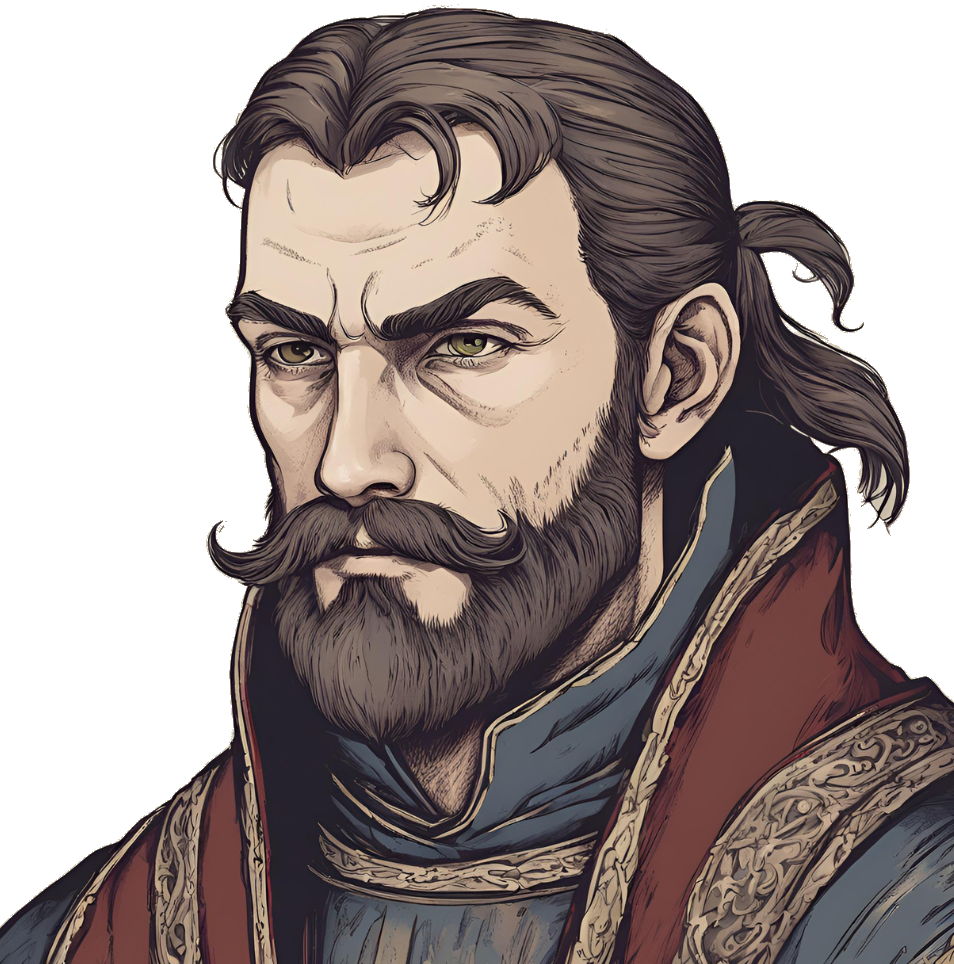
\includegraphics[width=7.5cm]{img/tobaldo-malatesta.png}
    \caption{\textsf{Tobaldo Malatesta, servitore di alto rango di Matilde di Canossa.\cite{url:ai}}}
    \label{fig:tobaldo}
\end{figure}

\begin{DndSidebar}{La missiva per Matilde}
Il DM dovrebbe stampare la lettera destinata a Matilde di Canossa, arrotolarla in stile pergamena o sigillarla con cera lacca e consegnarla fisicamente al giocatore che interpreta Dante Passafiume. Il fatto di avere una lettera chiusa in mano dovrebbe stimolare la curiosità dei giocatore e magari anche la tentazione di dare una sbirciatina. Oppure Herbert Mann potrebbe tentare di rubarla.
\end{DndSidebar}

\DndFeatHeader{Il carro al sicuro}
All'arrivo al villaggio di San Polo i PG saranno costretti ad alloggiare alla locanda per trascorrere la notte ed eventualmente attendere il passaggio della tormenta. Nella locanda troveranno alcuni NPC che racconteranno quanto il DM vorrà della storia riportata all'inizio del presente testo.

\begin{DndReadAloud}
Quando entrate nella locanda affollata, il brusio di abbassa istantaneamente e alcuni ospiti si girano per osservarvi incuriositi. La maggior parte di loro sono contadini. All'ingresso un misto di odore stufato, legna bruciata, letame e sudore arriva alle vostre narici. L'oste vi fa un caloroso sorriso dietro ai suoi baffoni e vi invita ad accomodarvi.
\end{DndReadAloud}

L'oste, Filippo Pocaterra (\textbf{popolano}) (Fig.\ref{fig:oste}), darà il massimo delle rassicurazioni ai PG garantendo che nessuno potrà toccare i viveri presenti sul carro in quanto saranno posizionati in una stalla che verrà chiusa con un pesante lucchetto.




\DndFeatHeader{NPC della locanda}
Alla locanda sono presenti alcuni abitanti della zona, per lo più contadini. Il DM potrebbe aggiungere eventuali PG che non partecipano alla OneShot tenendo conto del loro background. Ad esempio la cameriera potrebbe essere Isabella Grattaciotoli, nel caso non partecipi all'avventura come PG.

Alla locanda potranno parlare con persone della zona che li informeranno sul fatto che circola voce che Goffredo il Gobbo sia giunto dalla Francia per andare al Castello di Canossa per riconquistare Matilde. Se i PG non sono ancora stati informati sui fatti storici passati e che significato abbia la visita di Goffredo il Gobbo, il DM dovrebbe interpretare gli NPC per fornire ai giocatori le informazioni descritte nell'inquadramento storico riportato all'inizio del testo.

\DndFeatHeader{Il pasto}
L'oste offrirà loro una camera agiata è una sostanziosa cena al costo di 8 ma. Per la cena potranno scegliere fra stufato di maiale o brodetto di pernice e una caraffa di vino rosso.

I PG che mangeranno lo stufato di maiale, prima di coricarsi, dovranno fare un TS su costituzione con CD 11, se non lo superano, si ammaleranno di \textit{Epidemia fognaria} (Manuale del DM, p.257 \cite{dnd:dm})). I PG ammalati passeranno la notte vomitando e, il giorno dopo saranno \textit{Indeboliti} al livello 1 (Manuale del Giocatore p.291 \cite{dnd:giocatore}). Alla mattina potranno rifare un TS su costituzione per vedere se l'indebolimento peggiora o migliora. Al termine di ogni riposo lungo successivo, potranno rifare il TS per vedere se la malattia si aggrava o no, non potranno recuperare PF ma potranno tirare un dado vita ogni riposo breve di almeno 1 ora aggiungendo metà del punteggio ottenuto.

\begin{DndTable}[color=PhbLightCyan,header=Indebolimento]{cX}
  \textbf{Liv.} & \textbf{Effetto} \\
  1 & Svantaggio alle prove di caratteristica \\
  2 & Velocità dimezzata \\
  3 & Svantaggio ai tiri per colpire e ai TS \\
  4 & Massimo dei punti ferita dimezzato \\
  6 & Velocità ridotta a 0 \\
  7 & Morte \\
\end{DndTable}

\begin{figure}
\centering
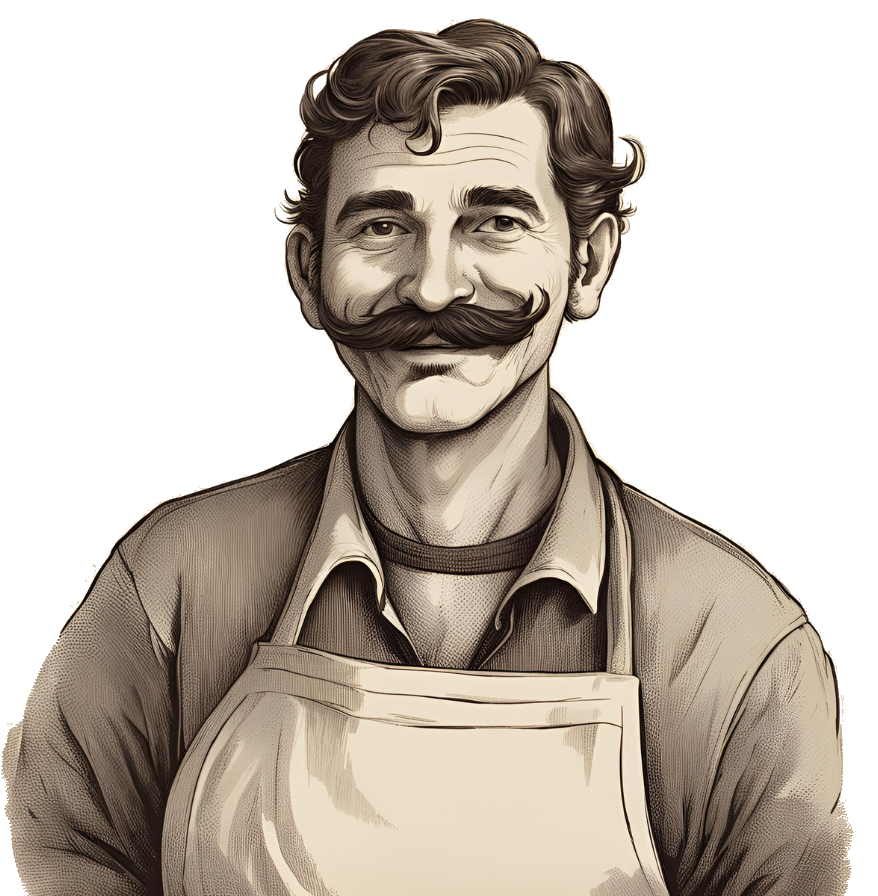
\includegraphics[width=7.5cm]{img/filippo-pocaterra.png}
    \caption{\textsf{Filippo Pocaterra, oste e proprietario della locanda Il cane zoppo a San Polo d'Enza.}\cite{url:ai}}
    \label{fig:oste}
\end{figure}




\chapter{Verso Canossa}
\DndDropCapLine{L}{a tormenta è passata.} I PG si risvegliano in una limpida giornata invernale. L'aria è fredda e luminosa, e il paesaggio è interamente coperto di neve. Guardando a nord, possono ammirare la foresta che si estende nella pianura, con le Alpi appena visibili sullo sfondo, anch'esse ricoperte di neve.

Quando i personaggi si metteranno in viaggio verso il Castello di Canossa, avranno due opzioni: possono dirigersi verso Quattro Castella e salire fino a Canossa, oppure proseguire lungo la valle dell'Enza e poi salire verso est per raggiungere Canossa..

\section{Incontri durante il viaggio}
Il DM potrà scegliere scegliere se inserire uno o più incontri: In questo testo viene presentato un incontro semplice adatto anche a giocatori alle prime armi.

\subsection{Imboscata}
I PG troveranno sul terreno un finto cadavere.

\begin{DndReadAloud}
Mentre proseguite sulla carraia coperta di neve in questa limpida giornata invernale, scorgete a terra qualcosa. Potrebbe sembrare un mucchio di panni o vestiti.
\end{DndReadAloud}

Mano a mano che i PG si avvicinano descrivi quanto segue:

\begin{DndReadAloud}
Ciò che inizialmente sembrava un ammasso di vestiti si trasforma progressivamente in una figura umanoide man mano che vi avvicinate. Da vicino, capite di essere di fronte a una creatura umanoide riversa a terra, con le braccia sotto il corpo in posizione prona e il volto nascosto nella neve. Diverse impronte conducono nel bosco sulla destra.
\end{DndReadAloud}

Facendo una prova a distanza su \textit{Indagare} con CD 16 potranno intuire che si tratta di un fantoccio. Se si avvicineranno al corpo per guardarlo da vicino, quando saranno a distanza sufficiente per capire che è un trucco per ingannarli, un \textbf{druido} (M.M. p.346) accompagnato da 2 \textbf{berseker} (M.M. p.244) sbucherà dal bosco e per prima cosa lancerà l'incantesimo \textit{Intralciare} su tutti i PG presenti vicino al cadavere (TS su Forza cd 12).

Successivamente colpiranno i berseker e il DM potrà far tirare per Iniziativa gli altri PG per iniziare la battaglia.







\section{Udienza con Matilde}
Quando i PG stanno per arrivare al Castello di Canossa, descrivi quanto segue.

\begin{figure}
\centering
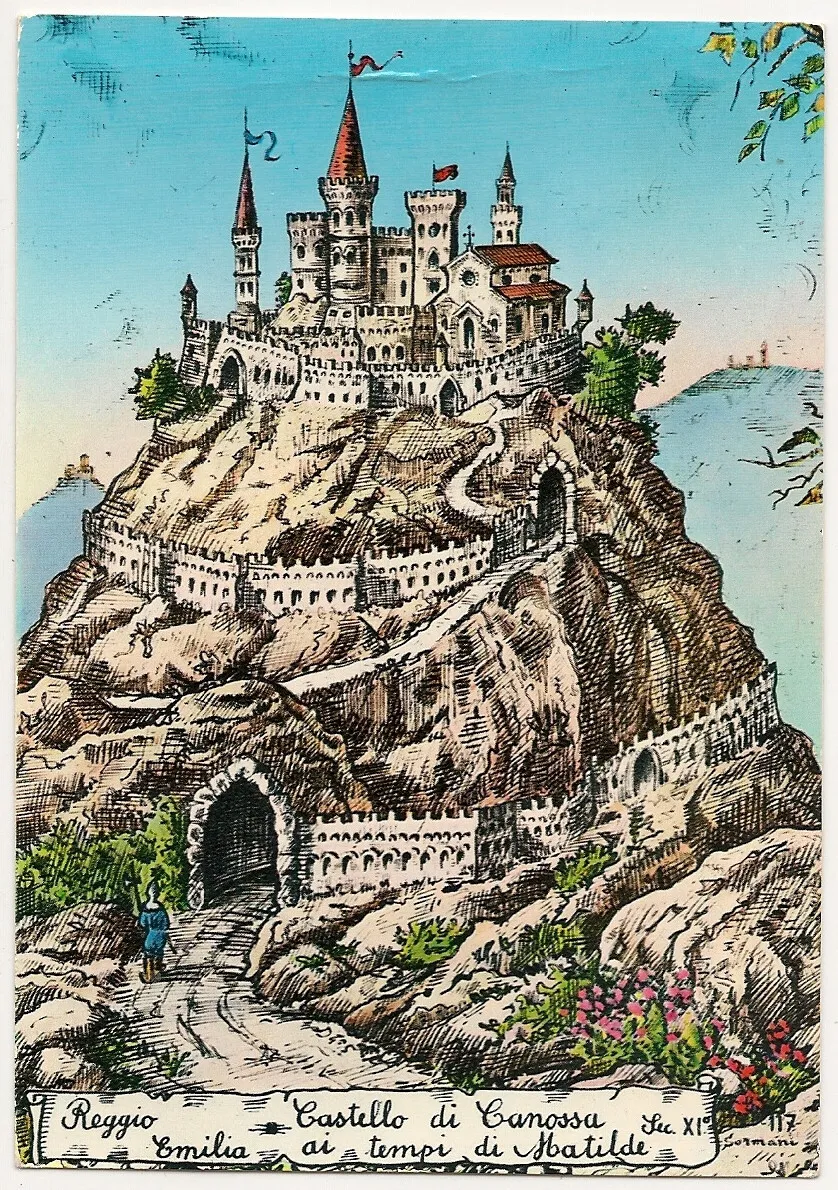
\includegraphics[width=7.5cm]{img/castello.png}
\caption{Il Castello di Canossa riprodotto in una cartolina pubblicata e in vendita su eBay}
\label{castello}
\end{figure}


\begin{DndReadAloud}
Mentre il carro tirato dal povero animale da soma procede lungo la mulattiera coperta di neve ogni tanto scorgente un promontorio di arenaria sul quale sorge il maestoso Castello di Canossa, residenza di Matilde. Mano a mano che procedete uscite dal bosco e potete scorgere l'intero paesaggio della zona. Nelle colline vicine a Canossa, in questa bella giornata d'inverno scorgete, su una collina vicina, la fortezza difensiva di Canossa: Rossena con la sua torre di guardia che molti chiamano Rossenella.

Quanto arrivate alla residenza di Matilde, alle porte delle mura che conducono al promontorio due \textbf{guardie} vi intimano di fermarvi. <<Alt! Chi siete? Cosa volete? Cosa portate?>>
\end{DndReadAloud}

%AGGIUNGERE DETTAGLI DEL CASTELLO DI CANOSSA
I PG potranno lasciare il carro nelle stalle che si trovano nei pressi delle dispense del castello. Dovranno aiutare il personale di servizio a scaricare i viveri e a disporli nelle cantine.

Non sarà facile per loro convincere le guardie che Dante dovrà consegnare personalmente la missiva a Matilde di Canossa. Il DM potrà ascoltare le motivazioni proposte dai giocatori ed eventualmente proporre delle prove su \textit{Persuasione}.

Matilde riceverà i PG nella sala delle udienze, leggerà la lettera e disperata la getterà a terra. Si spera che i giocatori a questo punto raccoglieranno la lettera per leggerla. Matilde e la madre Beatrice chiederanno l'aiuto dei PG per proteggere il Duca Goffredo e li faranno scortare fino la Castello di Rossena dove alloggia.

\chapter{Proteggere Goffredo}
\DndDropCapLine{D}{opo l'udienza con Matilde} i PG si recheranno al Castello di Rossena, roccaforte difensiva dell'area, per incontrare il Duca Goffredo III di Lorena detto "il Gobbo", \textbf{nobile}.

Il castello è presidiato da 15 \textbf{guardie}: 10 sono guardie della fortezza e 5 sono parte della scorta del Duca. Nella fortezza è presente anche Desiderio Montecucoli, un \textbf{veterano} il capo delle guardie di Rossena. Sono inoltre presenti 7 unità di personale di servizio fra cuochi e cameriere, \textbf{popolani}.

Goffredo sarà seccato dall'arrivo dei PG, ma soprattutto alterato poiché è stato rifiutato da Matilde nonostante le abbia promesso vasti territori ed eserciti. Matilde lo ha cacciato da Canossa, ma i consiglieri di Matilde hanno convinto la Contessa che, per non creare scandalo per la cacciata del Duca, sarebbe stato opportuno farlo alloggiare al Castello di Rossena in attesa della festa di fine anno, ma soprattutto in attesa che il Duca organizzi il suo viaggio di ritorno in Francia.

\section{Interpretare il Duca}
Il DM dovrebbe pensare a diversi impegni del Duca per movimentare la situazione e creare possibili situazioni di pericolo per la sua incolumità e opportunità per il PG infiltrato di fare le sue mosse. Il DM dovrà tenere presente che Goffredo è infastidito da questo controllo serrato su di lui e ci tiene molto alla sua privacy. Pertanto, tenderà sempre a chiudersi in una stanza anche per eventuali incontri o riunione lasciando i PG fuori.

Di seguito è presente una tabella con alcuni possibili impegni del Duca.

\begin{DndTable}[color=PhbLightCyan,header=Possibili impegni del Duca]{cX}
  \textbf{d4} & \textbf{Evento} \\
  1 & Incontro con il fratello per decidere come gestire il rifiuto di Matilde di Canossa \\
  2 & Una battuta di caccia a cavallo assieme al fratello \\
  3 & Pranzo nel salone per la lettura di documenti \\
  4 & Missione a Canossa per incontrare nuovamente Matilde \\
\end{DndTable}

\subsection{Il vicario}
Nel castello di Rossena i PG incontreranno Leonard Wormtongue, \textbf{drow mago} (M.M. p.129) di allineamento neutrale puro\footnote{A differenza di quanto indicato sul Manuale dei Mostri\cite{dnd:mostri} il drow mago in questione ha un allineamento neutrale puro. Anche se il DM dovrà cercare di far cadere qualche sospetto su di lui, Leonard non ha alcuna intenzione malvagia nei confronti dei PG e nemmeno nei confronti di Goffredo o Matilde}, vicario delegato da Matilde del Castello di Rossena. Il DM dovrebbe gestire questo NPC in modo ambiguo, cercando di far cadere qualche sospetto su di lui, ma senza esagerare. Lo scopo è spingere i PG ad indagare su Leonard ma giungere a conclusione che è una brava persona. Leonard non ha alcun interesse nell'uccidere Goffredo, è molto attento alla sua privacy e non esita ad utilizzare l'incantesimo \textit{Invisibilità superiore} per recarsi nella stanza di studio vicina alla camera di Goffredo ne caso fosse interdetta dai PG per ragioni di sicurezza al fine di proteggere Goffredo. Se Leonard venisse minacciato dai PG, userà l'incantesimo \textit{Camuffare se stesso} per farsi crescere artigli, zanne e corna sul proprio corpo (vedi M.d.G. p.212\cite{dnd:giocatore}).

\DndArea{Castello di Rossena}
Le seguenti descrizioni fanno riferimento alla figura \ref{rossena1} che rappresenta il Castello di Rossena. Questa planimetria non ha alcuna attinenza con la reale planimetria del castello, ma è stata costruita in modo utile a questa avventura.

\DndSubArea{Sala delle udienze} %a
\begin{DndReadAloud}
Vi trovate in un salone maestoso utilizzato dalla Contessa Matilde per incontrare i propri sudditi o nobili della zona come testimonia il trono posizionato su un tappeto rosso. Le pareti di questa sala sono decorate con arazzi e dipinti che rappresentano scene di caccia e ritratti di antenati della casata dei Canossa.

Sul trono è seduto un elfo scuro che vedendovi vi invita ad accomodarvi e si presenta. <<Buongiorno avventorieri. Leonard Wormtongue al vostro servizio>>. L'elfo si alza e fa un leggero inchino.
\end{DndReadAloud}

In questa sala sono presenti 5 \textbf{guardie}. Le guardie si riuniscono periodicamente in questa stanza per decidere le strategie di comando e gestione della fortezza.

Nell'angolo della stanza è presente una armatura di metallo.

Indagando sull'armatura i PG possono scoprire che l'armatura è appartenuta a Bonifacio, padre di Matilde.

Nell'angolo sud della stanza, è presente una scala che conduce al corridoio \textbf{n} del piano superiore.

\DndSubArea{Ingresso} %b
Sala d'attesa per i visitatori. Nella stanza è presente un tappeto con un tavolo, una libreria che contiene volumi inerenti battaglie e discendenze nobiliari dei Canossa.
Nella stanza sono anche presenti 2 \textbf{guardie}. In fondo alla stanza è presente una libreria che occupa tutta la parete. Nell'angolo sud ovest, un meccanismo basato sulla rimozione di una candela permette di aprire una porta segreta che conduce ai sotterranei del castello (area \textbf{o}) nei quali sono presenti gli alloggi delle guardie e della servitù. Il meccanismo può essere scoperto con una prova su \textit{Indagare} con CD 13.

\DndSubArea{Dispensa} %c
In questa dispensa sono presenti 2 barili di vino e un piccolo barile di aceto. Nelle scaffalature sono presenti cassette di verdure, formaggi, salumi stagionati e della cacciagione appena consegnata dai cacciatori della zona. Tutto il cibo è ottimo da mangiare. Qualunque prova effettuata dai PG confermerà che il cibo non ha problemi, a meno che qualcosa non intervenga per guastarlo o avvelenarlo.

\DndSubArea{Cucina} %d
In questa stanza, o nella dispensa adiacente, sono presenti 5 cuochi (\textbf{popolani}) impegnati a preparare il cibo per il pasto successivo. Ad esclusione della notte è sempre presente qualcuno che sta cucinando o comunque lavorando per preparare i pasti. Nella cucina sono presenti padelle, coltelli un acquaio e tutto quello che si può trovare in una cucina del Medioevo. È presente anche un barile di acqua potabile.

\DndSubArea{Sala} %e
Stanza di passaggio fra la cucina e il salone da pranzo. In questa stanza, oppure nella cucina o nella sala da pranzo sono presenti 2 cameriere (\textbf{popolane}) e 3 \textbf{guardie}.

\DndSubArea{Sala pranzo} %f
Un salone maestoso con un tavolo con 9 sedute. La tavola è sempre apparecchiata. In fondo alla sala è presente un camino con 2 poltrone e 2 armature in ferro.

\DndSubArea{Ripostiglio} %g
In questa stanza ci sono gli abiti del personale di servizio, attrezzi per la pulizia e altre cianfrusaglie.

\DndSubArea{Camera} %h
\begin{DndReadAloud}
Una camera spoglia con una latrina in fondo alla stanza che scarica direttamente sull'esterno del castello. Nella stanza è presente un letto matrimoniale in legno, un armadio, un'armatura di metallo e una sedia. Una pelle d'orso è posizionata al centro della stanza come tappeto. Nella stanza è anche presente un lavabo con una brocca d'acqua.
\end{DndReadAloud}
L'armadio ha al suo interno un passaggio segreto che conduce alla stanza \textbf{1c}. Può essere trovato con una prova su \textit{Indagare} CD 12. Goffredo, vorrà coricarsi spesso in questa stanza e utilizzerà la latrina presente nella stanza stessa. Goffredo non ha idea dell'esistenza del passaggio segreto.

\DndSubArea{Studio} %i
Questa stanza è uno studio, arredato con un tavolo sul quale sono posti alcuni libri e documenti, un armadio con all'interno dei cassetti, un camino, un baule, e una scaffalatura bassa sulla quale sono poste delle candele accese.
Se il Duca dovrà consultare dei documenti lo farà in questa stanza.

\DndSubArea{Stanza dei ricevimenti} %j
\begin{DndReadAloud}
Un grande tavolo in legno è collocato al centro della stanza probabilmente usata per riunioni e ricevimenti. Sotto al tavolo un bel tappeto finemente lavorato, sulla parete un armadio.
\end{DndReadAloud}
L'armadio contiene vestiti di fattura raffinata appesi a delle grucce, sul fondo dell'armadio si apre un passaggio segreto che conduce alla stanza \textbf{1h}. Il passaggio segreto può essere scoperto con una prova su \textit{Indagare} CD 12.
\DndSubArea{Ripostiglio} %k
In questa stanza ci sono mobili  rotti, sedie, tavoli e altri mobili in parte rotti accatastati. Se proveranno ad indagare potranno trovare dei documenti relativi ai possedimenti territoriali della casata dei Canossa, alcuni gioielli di poco valore, una corda, alcuni chiodi.

\DndSubArea{Stanza del camino} %l
In questa stanza è presente un camino spento e tutto quello che occorre per accendere il fuoco. Davanti al camino è un tappeto con due seggiole. Nella stanza è presente un'armatura di metallo e alcuni armadi.

\DndSubArea{Stanza da lettura} %m
\begin{DndReadAloud}
Al centro della stanza, sopra un tappeto di lana marrone, è presente un tavolo in legno tondo con intorno 4 sedie. Nella stessa stanza sono presenti un baule, e 3 armadi. Una piccola finestra illumina la stanza di luce naturale

Nell'armadio ad angolo sono presenti svariati testi storici che raccontano di battaglie, e testi religiosi. In mezzo ai testi è presente una pergamena sulla quale è scritto l'incantesimo da mago \textit{Trucco della corda} (Manuale del Giocatore p.287 \cite{dnd:giocatore}).
\end{DndReadAloud}

\DndSubArea{Corridoio e scale} %n
Scale e corridoio che conducono alla stanza \textbf{a}.

\DndSubArea{Camerata guardie}
Camerata delle guardie. Questa stanza comprende numerosi letti perfettamente rifatti delle guardie.

\DndSubArea{Camerata guardie}
Camerata delle guardie. Questa stanza comprende numerosi letti perfettamente rifatti delle guardie.

\DndSubArea{Corridoio fra le camerate}
Questa è una stanza di passaggio. Se i PG attraverseranno questo locale descrivi quanto segue.
\begin{DndReadAloud}
Una stanza di passaggio. Alle vostre spalla la porta che avete appena attraversato, di fronte a voi un altra porta. Sul pavimento un modesto tappeto e sulla destra una parete di armadi.

Quando percorrete la stanza, calpestando il tappeto il pavimento risuona in modo particolare.
\end{DndReadAloud}

Se i PG indagheranno sotto al tappeto troveranno una botola che conduce alla sala del tesoro \textbf{s}. Per accedere alla sala l dovranno superare un cancello.

\DndSubArea{Camerata della servitù}
Alcuni letti di fattura economica e un semplice armadio arredano la camera nella quale alloggia la servitù

\DndSubArea{Sala del tesoro}
Una sala contiene numerosi tesori accumulati
%COMPLETARE

\begin{figure*}
\centering
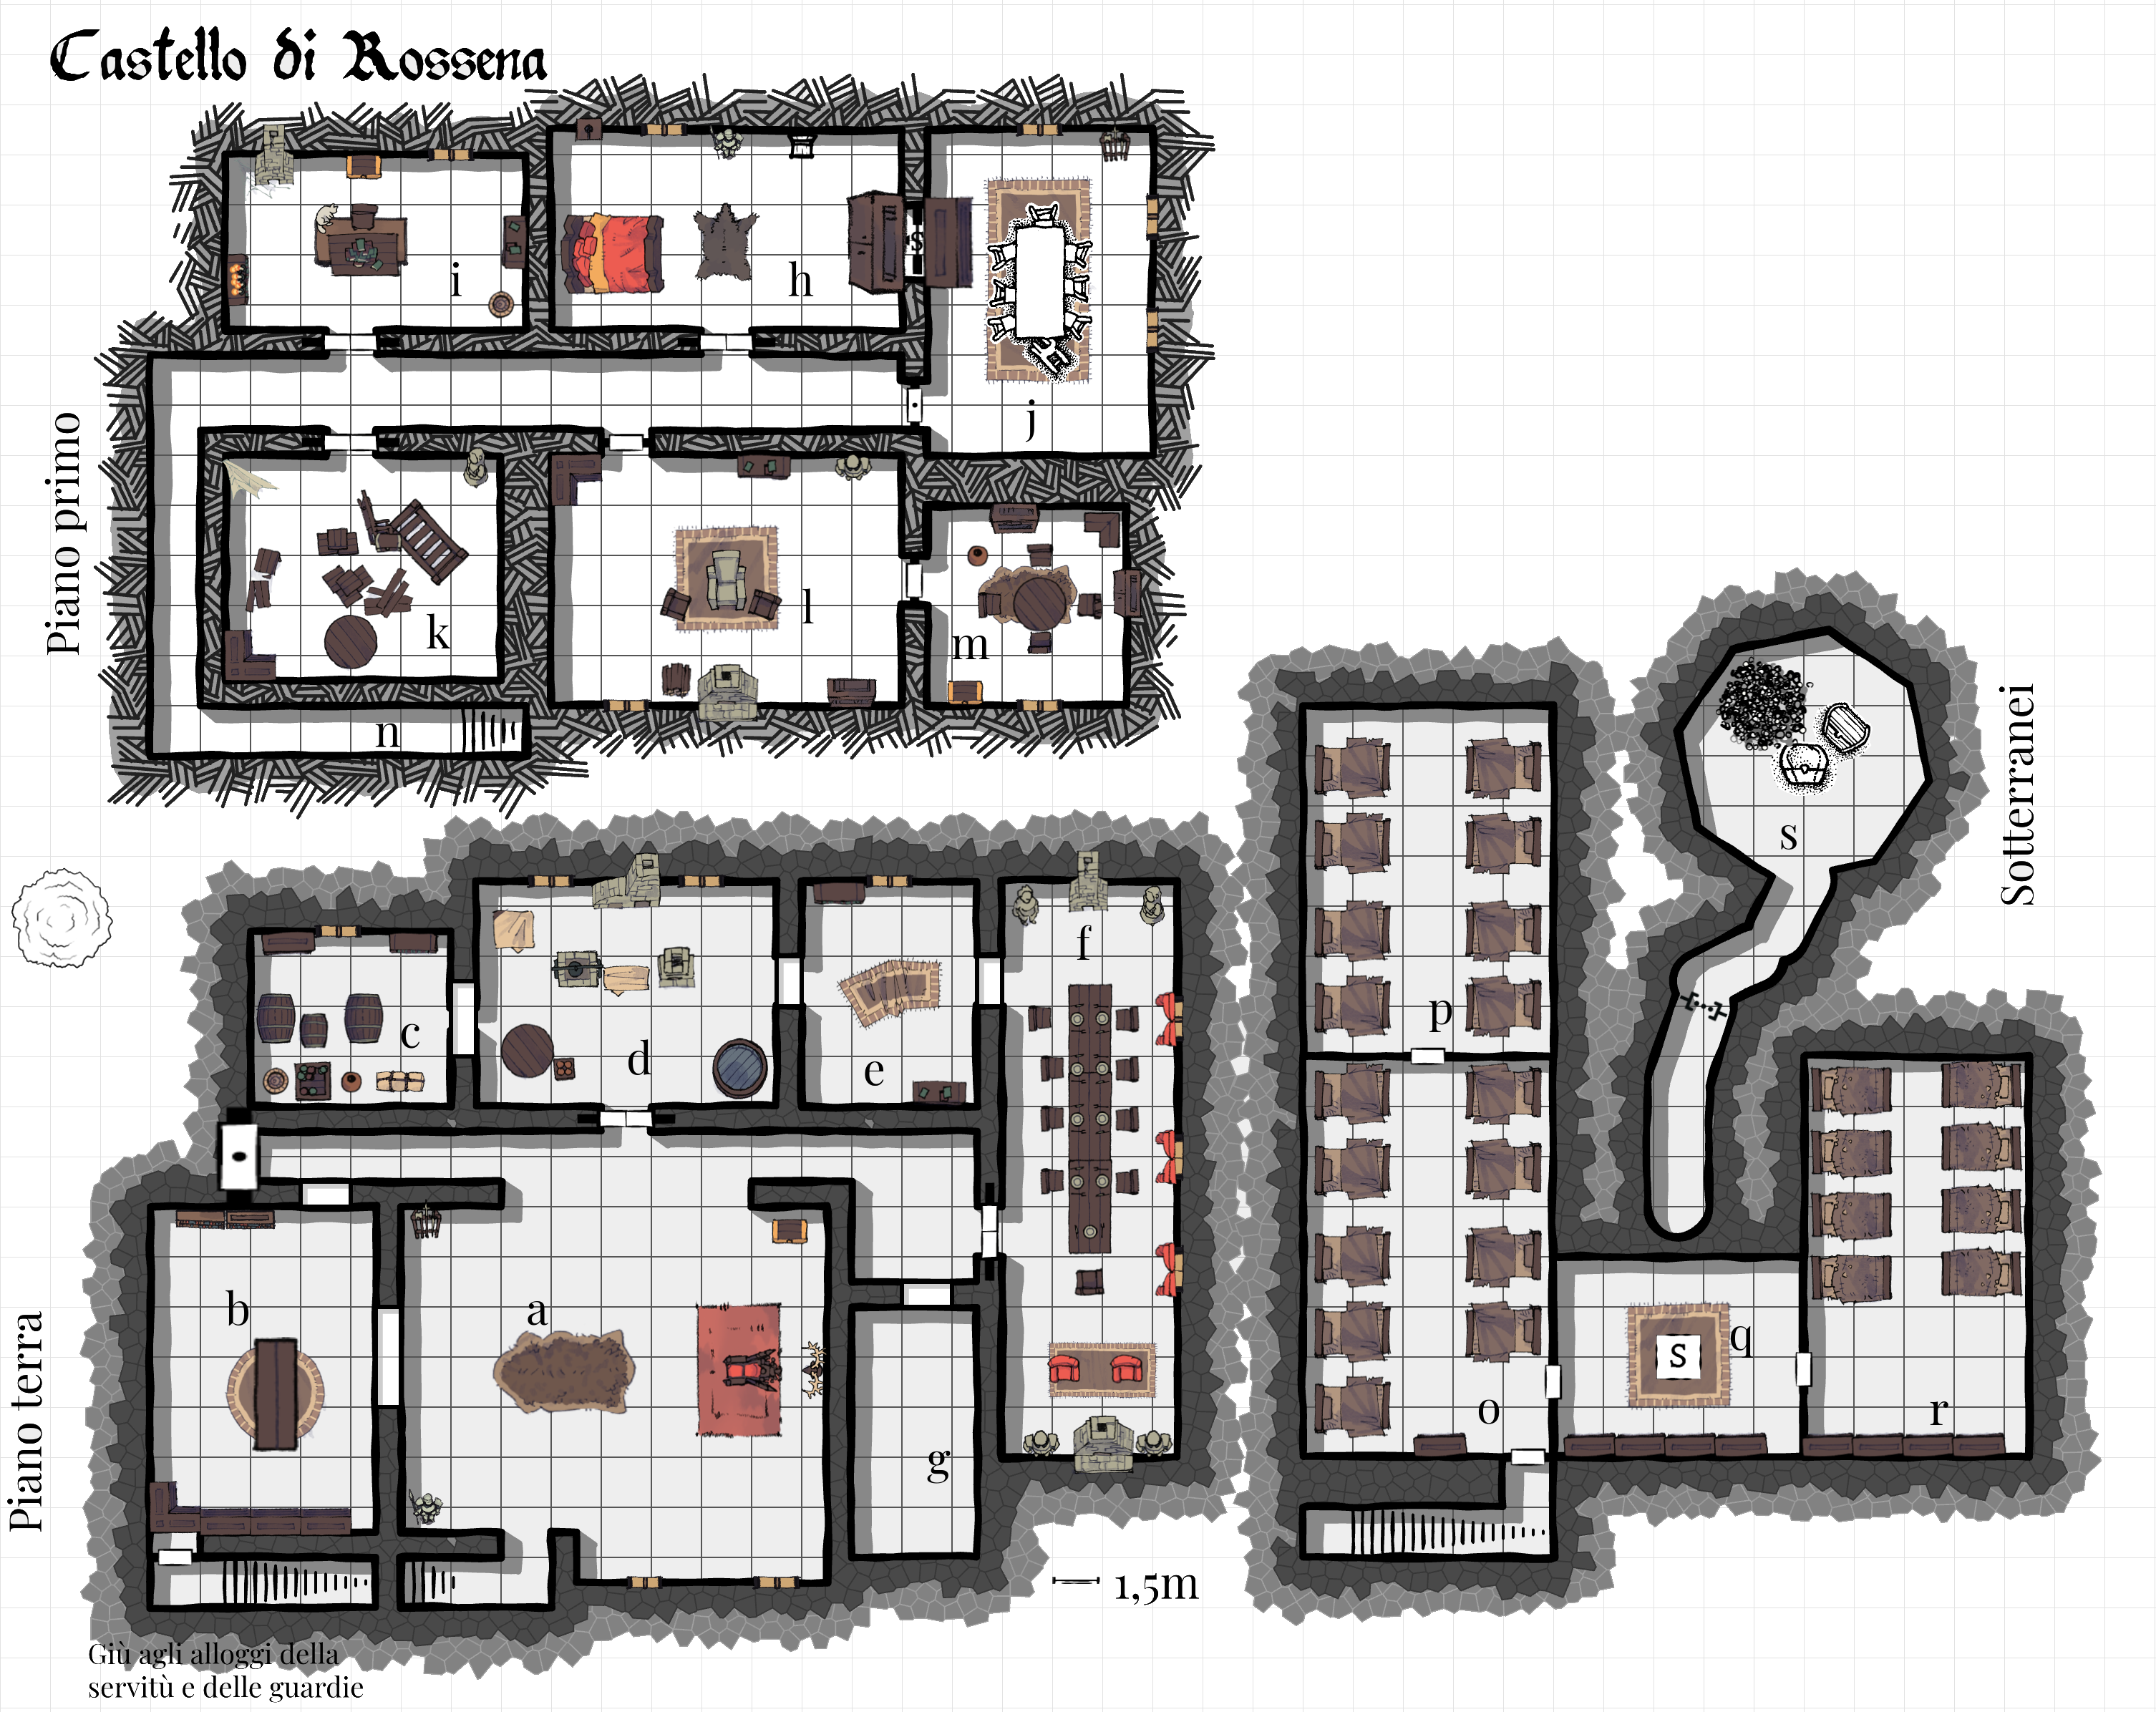
\includegraphics[width=0.9\textwidth]{img/rossena.png}
\caption{Planimetria del Castello di Rossena. Questa immagine è stata realizzata dagli scriventi ed è stata pubblicata come immagine di Pubblico Dominio su Wikimedia Commons. Un quadretto = 1,5m.}
\label{rossena1}
\end{figure*}


\chapter*{Licenza Creative Commons [CC-BY-SA]}
\subsubsection{Perché una licenza? Tiratela meno!}

Questa licenza (CC-BY-SA) è pensata per dare a chi utilizza questo testo maggiore libertà, dichiarandolo esplicitamente, non il contrario!! Puoi fare praticamente quello che vuoi di questo testo, compreso ripubblicarlo, l'unica limitazione che abbiamo aggiunto consiste nel fatto che, se apporti le modifiche al testo e desideri ripubblicarlo, dovresti farlo con la medesima licenza, in modo che anche altri possano divertirsi con il tuo lavoro!

\subsubsection{[CC BY-SA 4.0 Deed]}
Ad esclusione della sezione "Contesto storico" estratta da \textit{Wikipedia.org}, a cui si rimanda per la specifica licenza e alcune delle immagini (vedi didascalie), il presente testo è pubblicato con la licenza \textit{Creative Commons Attribuzione - Condividi allo stesso modo 4.0 Internazionale}.

\subsubsection{Tu sei libero di:}

    \textbf{Condividere} — riprodurre, distribuire, comunicare al pubblico, esporre in pubblico, rappresentare, eseguire e recitare questo materiale con qualsiasi mezzo e formato per qualsiasi fine, anche commerciale.
    
    \textbf{Modificare} — remixare, trasformare il materiale e basarti su di esso per le tue opere per qualsiasi fine, anche commerciale.
    Il licenziante non può revocare questi diritti fintanto che tu rispetti i termini della licenza.

\subsubsection{Alle seguenti condizioni:}

    \textbf{Attribuzione} — Devi riconoscere una menzione di paternità adeguata, fornire un link alla licenza e indicare se sono state effettuate delle modifiche . Puoi fare ciò in qualsiasi maniera ragionevole possibile, ma non con modalità tali da suggerire che il licenziante avalli te o il tuo utilizzo del materiale.
    
    \textbf{StessaLicenza} — Se remixi, trasformi il materiale o ti basi su di esso, devi distribuire i tuoi contributi con la stessa licenza del materiale originario.
    Divieto di restrizioni aggiuntive — Non puoi applicare termini legali o misure tecnologiche che impongano ad altri soggetti dei vincoli giuridici su quanto la licenza consente loro di fare.

\subsubsection{Note:}

Non sei tenuto a rispettare i termini della licenza per quelle componenti del materiale che siano in pubblico dominio o nei casi in cui il tuo utilizzo sia consentito da una eccezione o limitazione prevista dalla legge.

Non sono fornite garanzie. La licenza può non conferirti tutte le autorizzazioni necessarie per l'utilizzo che ti prefiggi. Ad esempio, diritti di terzi come i diritti all'immagine, alla riservatezza e i diritti morali potrebbero restringere gli usi che ti prefiggi sul materiale.

\subsubsection{Invia un feedback}
Se hai giocato l'avventura descritta in questo testo ci piacerebbe molto avere un feedback di come è stata la tua sessione. Hai apportato delle modifiche alle dinamiche descritte? I giocatori si sono divertiti? Sono capitati eventi particolari durante il gioco? Puoi farcelo sapere scrivendo a \textit{massimo@fsfe.org}.

\begin{figure}
\centering

\includegraphics[width=0.2\textwidth]{img/by-sa.png}
\end{figure}

\bibliography{bibliografia}{}
\bibliographystyle{plain}


\end{document}



